\documentclass[12pt,a4paper]{article}
\usepackage[utf8]{inputenc}
\usepackage[english]{babel}
\usepackage{enumerate}
\usepackage{amsmath}
\usepackage{amsfonts}
\usepackage{amssymb}
\usepackage{graphicx}
\usepackage{fourier}
\usepackage[left=2cm,right=2cm,top=2cm,bottom=2cm]{geometry}
\usepackage{commath}
\usepackage{cancel}
\usepackage{placeins}
\author{Juan Carlos Apitz, ID 012523821}
\title{STAT572 - Homework Assignment 2}
\begin{document}

\maketitle

\section*{In-Class Exercises}

\subsection*{Exercise 2: Generate a Random Sample from the Gamma(3,2)}

For this exercise I used the in-class procedure where first we randomly generate uniformly a number $0<u<1$. Then we choose $ x=min\bigr\{x: F(x)\geq u\bigr\}$. Where $F(x)$ is the CDF of the Gamma distribution with parameters $n=3$ and $\lambda=2$. Compared with the output from the MATLAB Gamma random sample generating function [command: $hist(gamrnd(3,2,1,1000))]$, we see that the proposed code works well. See figures \ref{inclassfig1}, \ref{inclassfig3} and \ref{inclassfig2} below.


\begin{figure}[ht!]
\begin{center}
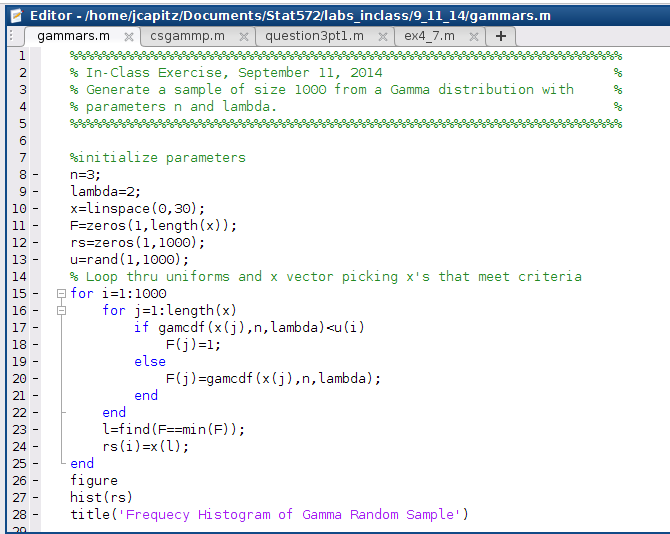
\includegraphics[scale=.60]{inClass_code.png}
\caption{Code of the in-class Gamma random sample exercise.}
\label{inclassfig1}
\end{center}
\end{figure}


\begin{figure}[ht!]
\begin{center}
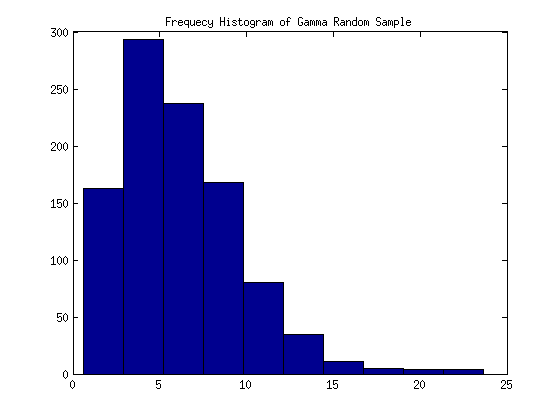
\includegraphics[scale=.80]{inClass_hist.png}
\caption{Histogram of the in-class Gamma random sample exercise, $n=3$ and $\lambda=2$.}
\label{inclassfig2}
\end{center}
\end{figure}

\begin{figure}[ht!]
\begin{center}
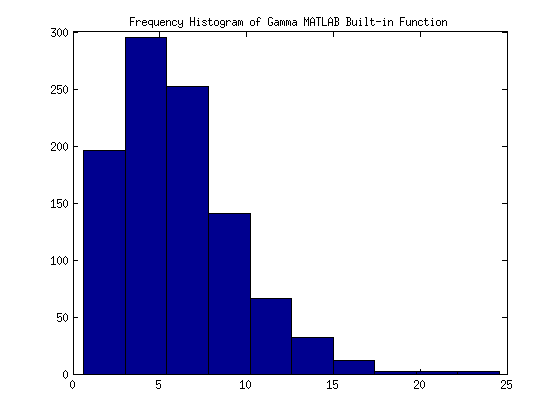
\includegraphics[scale=.80]{inClass_MATLABhist.png}
\caption{Histogram of a Gamma random sample generated by MATLAB's built-in function, $n=3$ and $\lambda=2$.}
\label{inclassfig3}
\end{center}
\end{figure}

\FloatBarrier

\section*{Homework 2}

\subsection*{Exercise 3.1}
\textbf{Code for Exercise 3.1 and 3.5.}
\begin{figure}[ht!]
\begin{center}
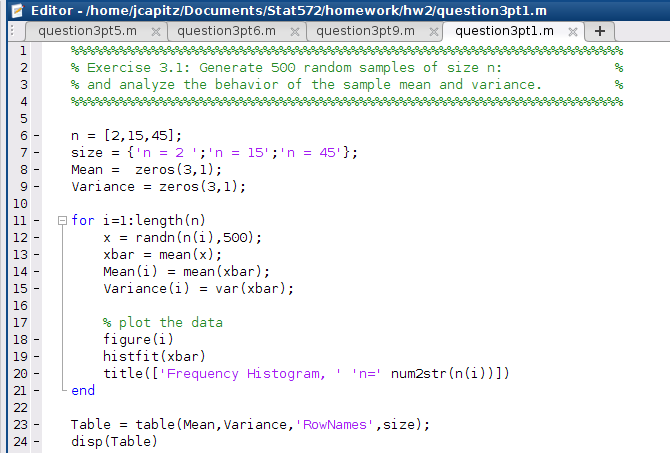
\includegraphics[scale=.50]{q3pt1_code.png}
\caption{Code Exercise 3.1.}
\label{q3pt1fig1}
\end{center}
\end{figure}
\FloatBarrier

\textbf{Discussion of Mean and Variance.}\\

In figure \ref{q3pt1fig2} below we can see the resulting values for the sample mean and sample variance of the calculated mean at each sample size. As predicted by the Central Limit Theorem, we see that the distribution of the sample mean, $\bar{x}$, looks approximately normal, the larger the sample size (see histograms,figure  \ref{q3pt1fig3}, \ref{q3pt1fig4}, and \ref{q3pt1fig5}). Additionally, we see that as $n$ gets larger, $\bar{x}$ approaches $\mu=0$, and $s_{\bar{x}}^2$ approaches $\frac{\sigma^2}{n}=\frac{1}{n}\rightarrow0$  the larger the sample size.  This is precisely what is predicted by CLT.\\

\begin{figure}[ht!]
\begin{center}
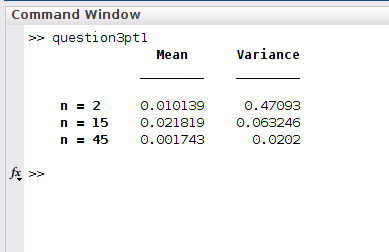
\includegraphics[scale=.80]{q3pt1_table.png}
\caption{Results, mean and variance.}
\label{q3pt1fig2}
\end{center}
\end{figure}
\FloatBarrier


\begin{figure}[ht!]
\begin{center}
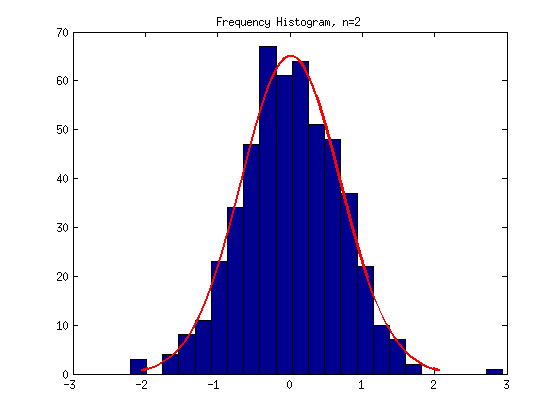
\includegraphics[scale=.70]{q3pt1_hist_2.png}
\caption{Frequency Histogram of Sample Means, n=2.}
\label{q3pt1fig3}
\end{center}
\end{figure}
\FloatBarrier

\begin{figure}[ht!]
\begin{center}
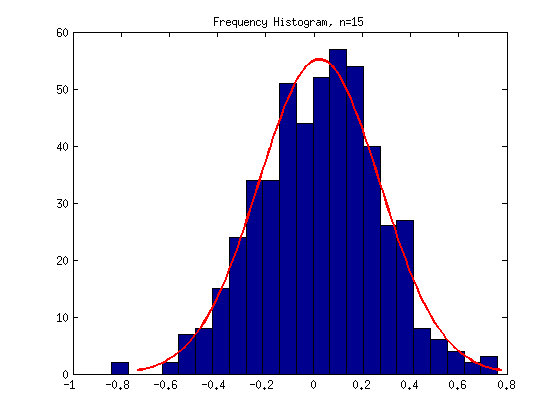
\includegraphics[scale=.70]{q3pt1_hist_15.png}
\caption{Frequency Histogram of Sample Means, n=15.}
\label{q3pt1fig4}
\end{center}
\end{figure}
\FloatBarrier

\begin{figure}[ht!]
\begin{center}
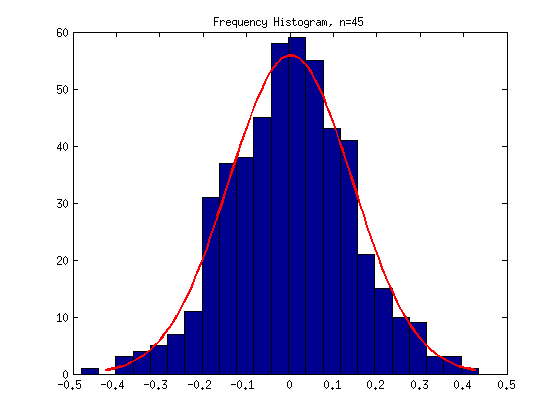
\includegraphics[scale=.70]{q3pt1_hist_45.png}
\caption{Frequency Histogram of Sample Means, n=45}
\label{q3pt1fig5}
\end{center}
\end{figure}
\FloatBarrier

\subsection*{Exercise 3.5}

\textbf{Discussion of Skewness and Kurtosis.}\\

In figure \ref{q3pt5fig1} we can see the results for the normal distribution's skewness and kurtosis . Since the data comes from a normal distribution, we expect the skewness coefficient to be near $0$ by symmetry. This is the case, specially when $n=45000$, which is expected as the larger the sample size the closer it will resemble its true distribution. The kurtosis of a normal distribution is in theory equal to 3. As we can observe in figure \ref{q3pt5fig1} the coefficient of kurtosis tends to 3.

\begin{figure}[ht!]
\begin{center}
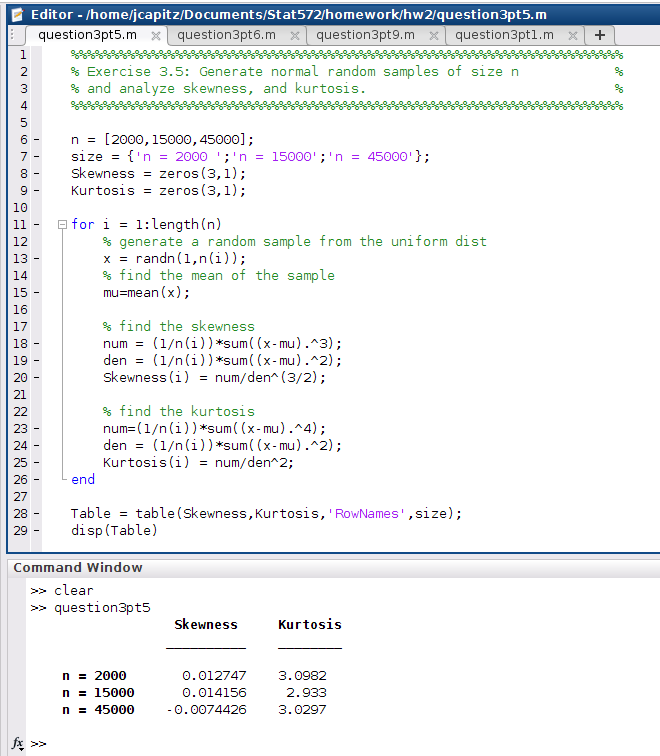
\includegraphics[scale=.60]{q3pt5_code.png}
\caption{Code and results for analysis of skewness and kurtosis - normal distribution.}
\label{q3pt5fig1}
\end{center}
\end{figure}
\FloatBarrier

\subsection*{Exercise 3.6}

\begin{figure}[ht!]
\begin{center}
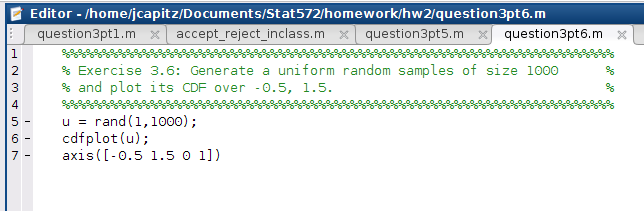
\includegraphics[scale=.50]{q3pt6_code.png}
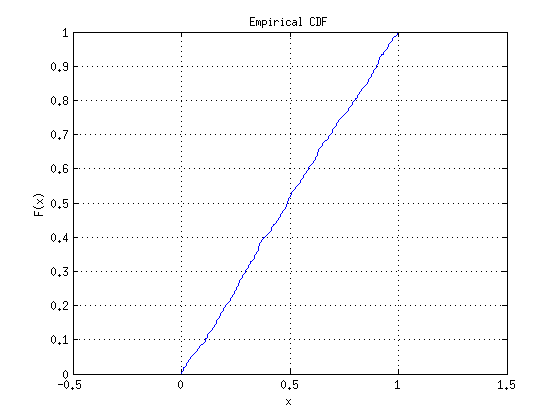
\includegraphics[scale=.70]{q3pt6_plot.png}
\caption{Code and CDF plot for uniform sample, $n=1000$.}
\label{q3pt6fig1}
\end{center}
\end{figure}
\FloatBarrier

\subsection*{Exercise 3.9}

\textbf{Quantile Estimation Discussion.}\\

In theory, we expect, that given a random variable $u\sim Unif(0,1)$, its $q_{33}=0.33$, $q_{40}=0.40$, $q_{63}=0.63$, $q_{90}=0.90$. In this exercise, we get estimates that are close to the theoretical results: $\hat{q}_{33}=0.3329$, $\hat{q}_{40}=0.4033$, $\hat{q}_{63}=0.6422$, $\hat{q}_{90}=0.859$. See figure \ref{q3pt9fig1} below for results.

\begin{figure}[ht!]
\begin{center}
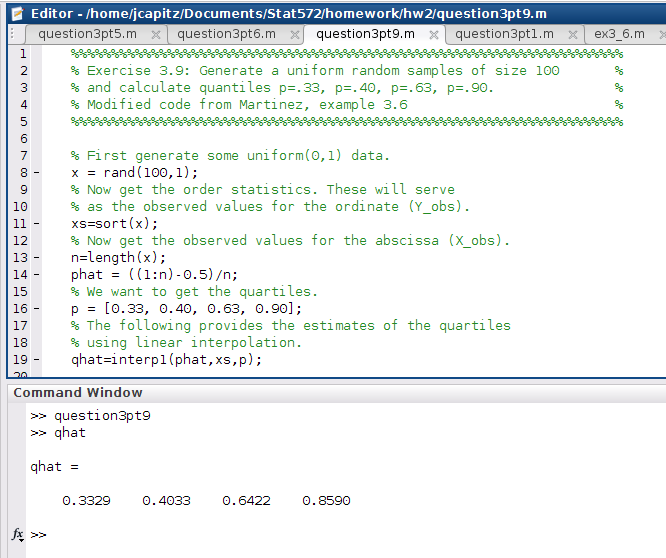
\includegraphics[scale=.60]{q3pt9_code.png}
\caption{}
\label{q3pt9fig1}
\end{center}
\end{figure}
\FloatBarrier

\subsection*{Exercise 3.11}

For this exercise I increased the sample size to $n=100,000$ for example $3.5$ and to $n=500,000$ for example 3.6. The results are shown in figure \ref{q3pt11fig1}. As we can see, these results are much closer to the true quartiles for both the Uniform and Normal distributions. For reference:\\

Uniform(0,1): $q_1=0.25$, $q_2=0.50$, $q_3=0.75$;\\

Normal(0,1): $q_1=-0.6745$, $q_2=0$, $q_3=0.6745$.\\


\begin{figure}[ht!]
\begin{center}
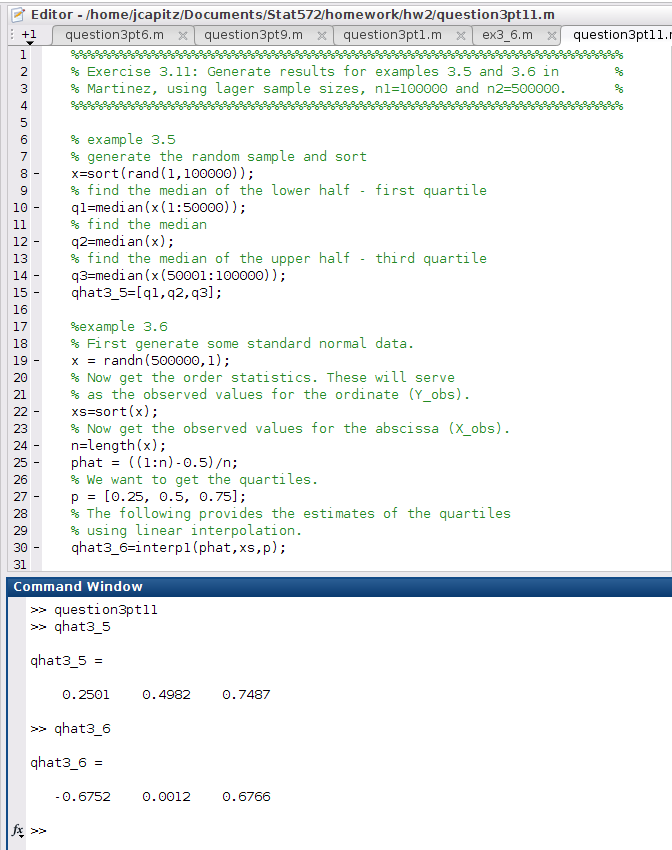
\includegraphics[scale=.60]{q3pt11_code.png}
\caption{}
\label{q3pt11fig1}
\end{center}
\end{figure}
\FloatBarrier

\subsection*{Exercise 3.16}

After completing the procedure required, the mean of the variances calculated is $0.998$, which gives us an absolute difference of  $\abs{0.998-1}=2.2202 \times 10^{-4}$, so very small. This is because I used a sample of size $5,000$ which makes the bias of the estimator very small. From mathematical statistics we know that the estimator  $S^2=\displaystyle\sum_{i=1}^n\dfrac{(x_i-\bar{x})^2}{n}$ has a bias of $\dfrac{n-1}{n}$ since $E\bigr(S^2\bigr)=\dfrac{n-1}{n}\sigma^2$.\\
For this exercise the theoretical value of the bias is $\dfrac{4999}{5000}=0.9998$ which precisely matches our our result, i.e. $E\bigr(S^2\bigr)=\dfrac{n-1}{n}\sigma^2=\dfrac{4999}{5000}\times1=0.9998$. See figure \ref{q3pt16fig1} below.

\begin{figure}[ht!]
\begin{center}
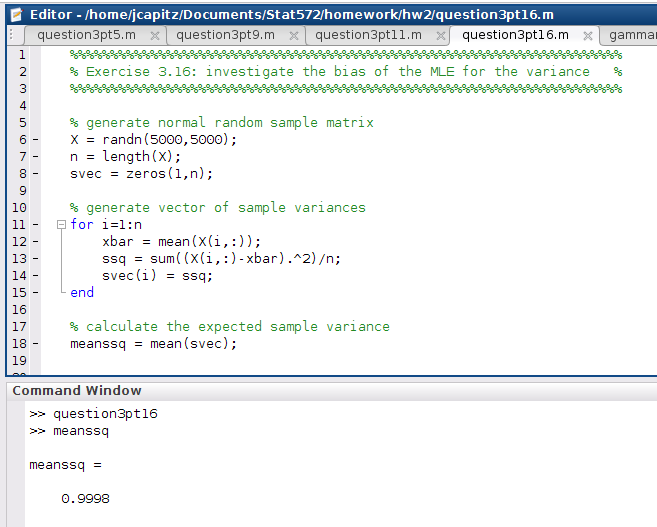
\includegraphics[scale=.60]{q3pt16_code.png}
\caption{}
\label{q3pt16fig1}
\end{center}
\end{figure}
\FloatBarrier

\end{document}